\section{Review of Wnt signaling}
\label{pathways:wnt}


\subsection{Brief overview of the Wnt signaling network}

Just as with \tgfbsf, Wnt signaling is morphogenic and is deeply conserved, having
orthologs in the basal metazoan \textit{Trichoplax adhaerens} \cite{Srivastava2008}.
Also like \tgfbsf, the Wnt pathway is essential to development, results
in highly context-dependent phenotypic outcomes, and is often
disregulated in disease. In most other respects, however, these two signaling
pathways are quite different. Wnt shares no core components with the \tgfbsf\
pathway, has many more components overall (and is thus more complex), and has
different kinetics. Finally, the mechanisms of
Wnt signal transduction are less understood and more contentious than are
the mechanisms of \tgfbsf\ signaling.


The ``canonical'' Wnt signaling pathway is
shown schematically in \autoref{fig:pathways:wnt}.
This pathway consists of diverse extracellular
Wnt ligands (\autoref{pathways:wnt:wnt}) that bind to 
FZD receptors (\autoref{pathways:wnt:frizzled}) and subsequently
cause stabilization of the transcription factor \bcat\
(\autoref{pathways:wnt:bcat}). As a result, concentrations
of nuclear \bcat\ increase and this protein can then take part in
highly context-dependent changes to the cellular transcriptional
program. In addition to this canonical signaling pathway, there
are many ``non-canonical'' Wnt pathways
(as many as ten! \cite{Malhotra2009}) that are poorly understood.
My focus in this dissertation is on canonical Wnt signaling, though
I briefly review non-canonical Wnt signaling below
(\autoref{pathways:wnt:noncanon}).


I note that the term ``canonical'' is falling out of favor
in the Wnt field, so that ``canonical Wnt pathway'' is being replaced by
``Wnt/\bcat\ pathway.'' I defined the term ``canonical'' somewhat differently
in \ar{introduction:introduction} to refer to a signaling network that is
relatively distinct from other networks. Indeed, such signaling insulation
is one of the aspects of Wnt/\bcat\ signaling that has made it easier to study
than other Wnt pathways. I therefore maintain the use of ``canonical'' to
refer to the Wnt/\bcat\ pathway in this dissertation, as
it carries with it the important connotation of independence. For simplicity,
by the shorthand ``Wnt signaling'' I always refer to the canonical variant
unless otherwise specified.



  \begin{figure}[!bt]
  \centering
  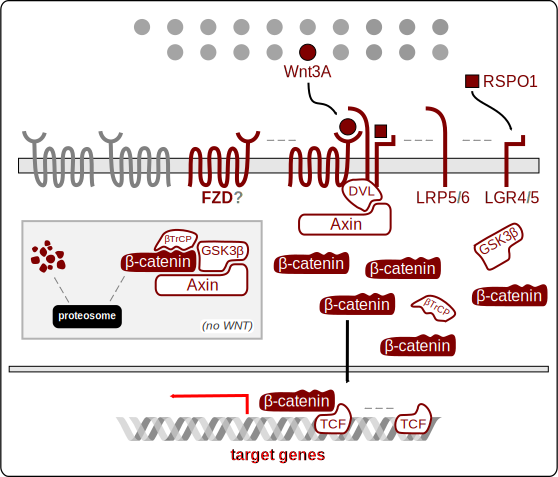
\includegraphics[width=4in]{FIGS/pathways/wnt.pdf}
  {\singlespacing 
  \caption[Structure of the canonical Wnt signaling pathway]
          {A simplified structure of the canonical Wnt signaling pathway.
          Of 19 ligands (circles), Wnt3A is the prototypical canonical ligand
          (filled red circle).
          Wnts binds to a subset of 10 FZDs, with a generally unknown degree
          of specificity. In the absence of
          Wnt (inset gray box), \bcat\ is proteosomally degraded after
          \pn\ and \ubn\ by the destruction
          complex. This complex includes the kinase \gsk, the E3 ubiquitin ligase
          \textbeta{TrCP}, and the scaffold Axin.
          In response to ligand, the destruction complex
          is disrupted in a Dishevelled (DVL)-dependent manner,
          allowing \bcat\ levels to accumulate.
          Nuclear \bcat\ binds to the co-factor TCF/Lef and together
          these factors modulate the transcriptional network of the cell.
  }
  \label{fig:pathways:wnt}}
  \end{figure}

  
  
  
  
  
\subsection{The Wnt ligands}
\label{pathways:wnt:wnt}


 \begin{figure}[!bt]
  \centering
  \includegraphics[width=4in]{FIGS/pathways/wnt_tree.pdf}
  {\singlespacing 
  \caption[Wnt pathway phylogenetic trees]
    { Phylogeny of the Wnt
      ligands (\textbf{a}, \autoref{pathways:wnt:wnt}),
      receptors (\textbf{b}, \autoref{pathways:wnt:frizzled}), and
      transcription factors (\textbf{c}, \autoref{pathways:wnt:bcat}).
      The \textit{T.a.} prefix indicates putative \ta\ proteins (gray).
      WG (Wingless), FZ (Frizzled), and ARM (Armadillo) are \fly\ orthologs
      of mammalian Wnt1, FZDs, and \bcat.
      JUP, Junctional Plakoglobin (also known as \textgamma-catenin)
      is a paralog of \bcat.
	  CTNNB1, gene symbol for \bcat.
      4F0A.B/A, identifiers for crystal structures of \frog\ Wnt8A
      and FZD8 used in the alignments. Wnt3A and Wnt5A (reds) are the
      prototypical canonical and non-canonical Wnt ligands, respectively. 
      As with the \tgfbsf\ pathway, note the high degree of diversity
      for each node when considering the basal \glspl{ta} proteins, and
      that the Wnts and FZDs each fall into multiple distinct subfamilies.
      Distances are approximate, in arbitrary length units
      (see \nameref{pathways:methods}).}
  \label{fig:wnt:trees}}
  \end{figure}



The mammalian Wnt ligands were initially identified with the discovery
of mouse Int-1, which was later found to be homologous to the \fly\
protein Wingless (WG). Mice are, of course,
wingless by default, and so in mammals these two gene names
were concatenated into the meaningless ``Wnt1.'' All other Wnt ligands
are named similarly \cite{Mikels2006}. In mammals, there are a total of
19 Wnts that fall into
multiple subfamilies by sequence homology (\autoref{fig:wnt:trees})
\cite{Clevers2006,Malhotra2009}. 


These small ligands ($\sim$350 amino acids) are highly cysteine-rich,
with 22 cysteine residues that have
conserved spacing across all Wnts. The evolutionary maintenance of these cysteines
was taken to imply the formation of intramolecular cysteine bridges, which suggested
that Wnt ligands should be stable proteins \cite{Mason1992}.
Further, aspects of the primary sequence, including many
charged residues, were suggestive of a protein that should be highly soluble.
Despite the expected stability and solubility of the Wnt ligands, they proved
to be quite problematic to work with \cite{Verheyen2010}.


In overexpression systems, intracellular Wnts were found to have many glycosylated forms and
tended to associate with chaperones, implying some difficulty in properly folding 
these proteins. Extracellular Wnts, in contrast, were found to have fewer glycosylated forms.
Further, the bulk of overexpressed Wnt products tended to remain in the cell \cite{Mikels2006},
and the Wnt proteins that left the cell tended to stay associated with membranes or with the
extracellular matrix \cite{Reichsman1996}. All of this data suggested that the Wnt
ligands were in fact neither stable nor soluble, explaining in part
the difficulty in purifying these proteins.


With the first successful purification of a functional Wnt in
2003, the explanation for the lack of solubility became clear: Wnts have an absolutely
conserved palmitoylated cysteine at the N-terminus. This lipidation is essential, as
mutant proteins lacking the lipidated cysteine
are incapable of signaling \cite{Willert2003}.
The relative insolubility of Wnt ligands have made them quite difficult to purify.
Indeed, purified Wnts are commercially available primarily through a single vendor
(R\&D Biosystems), and at
relatively low purity. As I show later in \autoref{insulation:system}
(\ar{fig:insulation:contamination}), this
low purity of the common reagent has important consequences to interpretation of
some experimental results.


To reduce experimental costs, studies therefore
frequently use Wnt-conditioned media instead of purified Wnts.
This approach suffers in that conditioned media contains a large amount of
unknown secreted cellular products. Cell lines that lack the Wnt
overexpression are often used as negative controls. However, given the degree of
transcriptional remodeling that the Wnt pathway can cause, there are likely
many unknown differences between Wnt-conditioned and control-conditioned
media.


The solubility problem for the Wnt ligands led to an additional difficulty,
that of determination of the tertiary structure of these proteins. Indeed, the first 
crystal structure of a Wnt was obtained only recently \cite{Janda2012}. The
primary sequence of Wnts are not related to any known protein fold, so prior
to the crystal structure there were many unknowns regarding how Wnts bind
to their various receptors and co-receptors. I touch on this more below.


    \begin{table}[!bt]
    \centering
	\footnotesize
    \caption[List of Wnt ligands]
            { Sequence sources for the 
              Wnt alignments in \autoref{fig:wnt:trees}. }
    \label{table:pathways:methods:wnt}
    \begin{tabular}{llll}
    \hline
    Symbol    & Species & NCBI GI & Accession \\ \hline
	Wnt1   & \textit{H. sapiens} & 4885655   & NP\_005421.1    \\
	Wnt2   & \textit{H. sapiens} & 4507927   & NP\_003382.1    \\
	Wnt2B  & \textit{H. sapiens} & 630044901 & NP\_001278809.1 \\
	Wnt3   & \textit{H. sapiens} & 13540477  & NP\_110380.1    \\
	Wnt3A  & \textit{H. sapiens} & 14916475  & NP\_149122.1    \\
	Wnt4   & \textit{H. sapiens} & 17402922  & NP\_110388.2    \\
	Wnt5A  & \textit{H. sapiens} & 371502087 & NP\_001243034.1 \\
	Wnt5B  & \textit{H. sapiens} & 17402919  & NP\_110402.2    \\
	Wnt6   & \textit{H. sapiens} & 16507239  & NP\_006513.1    \\
	Wnt7A  & \textit{H. sapiens} & 17505191  & NP\_004616.2    \\
	Wnt7B  & \textit{H. sapiens} & 17505193  & NP\_478679.1    \\
	Wnt8A  & \textit{H. sapiens} & 17505195  & NP\_490645.1    \\
	Wnt8B  & \textit{H. sapiens} & 110735437 & NP\_003384.2    \\
	Wnt9A  & \textit{H. sapiens} & 15082261  & NP\_003386.1    \\
	Wnt9B  & \textit{H. sapiens} & 17017976  & NP\_003387.1    \\
	Wnt10A & \textit{H. sapiens} & 16936520  & NP\_079492.2    \\
	Wnt10B & \textit{H. sapiens} & 16936522  & NP\_003385.2    \\
	Wnt11  & \textit{H. sapiens} & 17017974  & NP\_004617.2    \\
	Wnt16  & \textit{H. sapiens} & 17402914  & NP\_057171.2    \\
	WG     & \textit{D. melanogaster} & 17648113  & NP\_523502.1   \\
	T.a.30370& \textit{T. adhaerens}  & 196012489 & XP\_002116107.1 \\
	T.a.52489& \textit{T. adhaerens}  & 195996709 & XP\_002108223.1 \\ 
    \hline
    \end{tabular}
    \end{table}


	
	
	
	
	
	
\subsection{The Frizzled receptors}
\label{pathways:wnt:frizzled}



There are 10 human Wnt receptors, the Frizzleds (FZDs).
These are a diverse group of seven-pass G-coupled
protein receptors (GPCRs), though canonical signaling is mediated
primarily by non-G-protein mechanisms \cite{Angers2009}.
Upon binding to Wnt and various cofactors
the Wnt/FZD complex is likely endocytosed and
sequestered into multivesicular bodies within the cell. This receptor
internalization is essential to proper signaling
\cite{MacDonald2009,Taelman2010}. As a consequence of Wnt binding
to the Frizzled receptors, the transcription factor \bcat\
is stabilized. However, to date there are many competing
models and no clear front-runner for how FZD causes this outcome
(see \autoref{pathways:wnt:bcat}).


Essential for Wnt signaling through FZDs are the single-pass
transmembrane co-receptors, LRP5 and LRP6 (tongue-twistingly
expanding to ``Low-density lipoprotein receptor-related protein'' 5 and 6)
\cite{Clevers2006}. The ectodomain structure of LRP6 was recently
solved, revealing four tandem
beta-propellar-EGF-like domains that provide a large interface
for interacting proteins. Prior mutational studies of these domains
showed that they are essential for Wnt binding. Further, Dickkopf-1
(DKK1), a classical extracellular Wnt antagonist, was shown to bind
to these same domains, which would likely occlude the Wnt binding interface
\cite{Chen2011,Ahn2011,Cheng2011}. (I use purified DKK1 in
\ar{insulation:system} to demonstrate specificity of Wnt responses.)


Additional co-factors that are not essential but that dramatically
amplify Wnt signaling are the soluble protein R-spondin 1 (RSPO1)
\cite{Kim2005} and 
another subfamily of GPCRs, LGR4 and LGR5
(short for ``Leucine-rich repeat-containing G-protein coupled receptor
4 and 5''). It was recently discovered that these two co-factors
are themselves likely a ligand-receptor pair
\cite{Kim2005,Glinka2011,DeLau2011}, though the mechanism by which these co-factors
enhance Wnt signaling is still a mystery.


With ten receptors and multiple co-factors, we are left with the issue of
signaling specificity.
Wnts appear to have high promiscuity for the \fz s, with little
certainty in the field regarding which, if any, receptor-ligand pairings are excluded.
It is still unknown which Wnts bind to
which \fz s, or if \fz s can generally signal in both canonical and non-canonical ways
\cite{Angers2009,VanAmerongen2012}.
Unfortunately, while Wnt3A and Wnt5A are generally
considered to be the prototypical ligands for canonical and non-canonical
Wnt signaling, respectively  \cite{Huang2004}, there is
evidence that each can transduce signals through a non-prototypical pathway
under certain conditions \cite{VanAmerongen2012}.
The recent crystal structure of \frog\ Wnt8 with FZD8
did little to enhance our
understanding of the origins of receptor-ligand specificity,
as the intra-protein contacts occurred primarily at highly conserved
Wnt residues \cite{Janda2012}. This is suggestive that there is either
little specificity between ligands and receptors, or that specificity
is a more complicated outcome of interactions with other factors.




    \begin{table}[!bt]
    \centering
	\footnotesize
    \caption[List of Frizzleds]{ Sequence sources for the 
    Frizzled (FZD) alignments in \autoref{fig:wnt:trees}. }
    \label{table:pathways:methods:frizzled}
    \begin{tabular}{llll}
    \hline
    Symbol & Species & NCBI GI & Accession \\ \hline
	FZD1  & \textit{H. sapiens} & 4503825   & NP\_003496.1    \\ 
	FZD2  & \textit{H. sapiens} & 4503827   & NP\_001457.1    \\ 
	FZD3  & \textit{H. sapiens} & 8393378   & NP\_059108.1    \\ 
	FZD4  & \textit{H. sapiens} & 22547161  & NP\_036325.2    \\ 
	FZD5  & \textit{H. sapiens} & 27894385  & NP\_003459.2    \\ 
	FZD6  & \textit{H. sapiens} & 257470999 & NP\_001158087.1 \\ 
	FZD7  & \textit{H. sapiens} & 4503833   & NP\_003498.1    \\ 
	FZD8  & \textit{H. sapiens} & 13994190  & NP\_114072.1    \\ 
	FZD9  & \textit{H. sapiens} & 4503835   & NP\_003499.1    \\ 
	FZD10 & \textit{H. sapiens} & 6005762   & NP\_009128.1    \\ 
	FZ    & \textit{D. melanogaster}  & 17864440  & NP\_524812.1 \\
	T.a.12196 & \textit{T. adhaerens} & 196002269 & XP\_002111002.1 \\
	T.a.31674 & \textit{T. adhaerens} & 196014261 & XP\_002116990.1 \\
    \hline
    \end{tabular}
    \end{table}

	

\subsection{\bcat, the canonical Wnt effector}
\label{pathways:wnt:bcat}


\bcat\ is the main effector of canonical Wnt signaling. This
large protein is one of several catenins that are
used in cellular adhesion. \bcat\ itself has a large
membrane-associated pool dedicated to this task \cite{Jamieson2012}, while only a
``vanishingly small'' baseline cytosolic component is found
in Wnt un-stimulated cells \cite{Li2012}.


In the classic model of Wnt signaling, basal
\bcat\ is constitutively transcribed and translated, but then degraded
just as quickly in the absence of Wnt. Wnt stimulation stabilizes
\bcat, thus allowing cytosolic levels to build. In some systems,
cytosolic \bcat\ accumulation is measureable in as little as 15 minutes,
and reaches a stable peak response by 2 hours that can last longer
than 24 hours \cite{Li2012,Hernandez2012}.
The nuclear import/export rates for \bcat\ are unaffected by signaling,
and so it appears that nuclear accumulation resulting from Wnt 
signaling is due to an
overall change in protein abundance throughout the entire cell 
\cite{MacDonald2009,Clevers2006}.


Importantly, \bcat\ appears to encode information about extracellular
Wnt concentrations primarily in its nuclear concentration, as opposed to the
concentration of particular phosphorylation states. While various \bcat\ 
phospho-states have been discovered and claimed to
be required for the transcriptional activity of this protein, careful
quantification of post-signaling protein levels revealed that the vast
majority of \bcat\ is not phosphorylated in the presence of Wnt. Instead,
the phospho-state ends up at similar concentrations to the basal state \cite{Hernandez2012},
implying that phospho-\bcat\ does not encode Wnt ligand concentrations.


It is interesting to note that, like with the \tgfbsf\ pathways, the large
number of ligands and receptors end up bottlenecking to a small number of
effectors. This bottlenecking is more dramatic in the case of Wnt, as there
is only one \bcat\ gene to which all canonical Wnt signaling leads.
There is a highly homologous paralog, \textgamma-catenin
(also called Junctional Plakoglobin, JUP),
that differs from \bcat\ to a similar degree as does the functionally identical
\fly\ ortholog, Armadillo (see \autoref{fig:wnt:trees}). \textgamma-catenin
appears to have some functional redundancy to \bcat, and even after deletion of
both catenins some Wnt signaling has still been shown \cite{Malhotra2009}.
However, it appears that \bcat\ is the primary mediator of canonical Wnt
signaling. Interestingly, similarly to the \tgfbsf\ pathways described
earlier, this severe bottleneck implies that cells cannot
know which Wnt or Frizzled activated the pathway, unless an additional channel
of signaling carries this information.


To enact its transcriptional functions, accumulated nuclear
\bcat\ partners with one of a set of transcription
factors in the TCF/Lef family (standing for T-Cell Factor/Lymphoid 
enhancer-binding factor). There are four such proteins in mammals
that appear to be functionally redundant but do have different expression
patterns \cite{Clevers2006}. These are TCF7, TCF7L1, TCF7L2, and LEF1.
TCF1 was first discovered as a factor involved
with T-cell differentiation (hence the name) \cite{VandeWetering1991}, and later
connected to Wnt signaling after finding that a \frog\ ortholog, Xtcf-3,
could cause \bcat\ nuclear translocation \cite{MOLENAAR1996}.
TCF/Lef is normally bound to the protein Groucho, which prevents association of TCF/Lef
with \bcat. This block is lifted in response to Wnt signaling after \ubn\
of Groucho by XIAP (X-linked inhibitor of apoptosis) \cite{Hanson2012}.
It has been proposed that TCF/Lef binding to \bcat\ is stable enough to
effectively sequester it in the nucleus
and so allow for long-term Wnt signaling \cite{Jamieson2012},
though to my knowledge this has not been explicitly tested.


In complex with TCF/Lef, nuclear \bcat\ is able to bind to a diverse set of
promoters and modulate transcription. These targets are highly context-dependent,
though the negative auto-regulator Axin2 is considered to be a conserved
target of \bcat\ \cite{Clevers2006,Hatzis2008}. All canonical Wnt signals
are encoded into nuclear \bcat\ concentrations, therefore ligand-
and receptor-specific information must be lost during signal transduction.
This implies that the context-dependency of Wnt signaling responses should
be the result of transcriptional idiosyncrasies or of additional information
channels (e.g. non-canonical Wnt pathways).


\subsection{The destruction complex}
\label{pathways:wnt:destruction}


The functional effect of FZD, after binding Wnt,
is to relieve the otherwise constitutive degradation of \bcat. 
The set of proteins that are involved
with \bcat\ degradation is referred to, ominously,
as the ``destruction complex.'' The mechanisms by which this
complex degrades \bcat\ are fairly well understood, but how
active FZD causes an end to the destruction is still
highly contentious \cite{Hernandez2012,Li2012}.
Here, I discuss the components of this
complex that are best understood, and that will become important
later in the discussion on crosstalk between Wnt and \tgfbsf\
(\ar{pathways:wntTgfb:mechanism}).


\subsubsection{\gsk}

The protein Glycogen synthase kinase 3 beta (\gsk) maintains
a central role in the destruction complex. In fact, \gsk\ is
a signaling hub for many pathways, making it a prime node
for signal integration. \gsk\ is inhibited by Insulin and
growth factor signaling, which lead to phosphorylation of its N-terminal
tail. The phosphorylated tail becomes a ``pseudo-substrate'' that competes with the
actual substrates of \gsk. However, while this mechanism of inhibition
is well established, it is not clear if it is used by the Wnt
pathway. Nor is it clear whether the Wnt pathway maintains
a distinct pool of \gsk\ from growth factor pathways that can act
as an insulated information channel. If not, then modulation of a
common pool of \gsk\ by Wnt or other pathways would necessarily
create inter-pathway crosstalk.


What is clear is that this kinase requires ``priming'' phosphorylation
by another member of the \bcat\ destruction complex,
Casein Kinase 1 alpha (CK1\textalpha). This priming stems from phosphorylation 
of \bcat\ by CK1\textalpha, which produces a recognition site for subsequent
phosphorylation of \bcat\ by \gsk. Phosphorylation by
\gsk\ in turn creates a recognition site for the the ubiquitin E3 ligase
BTRC (beta-transducin repeat-containing protein, also known as \textbeta{TrCP}),
which subsequently ubiquitinates \bcat\ and sends it
off to the grinding mill of the proteosome
\cite{Frame2001,Hernandez2012}. The widely described model of
Wnt signaling has this \gsk-mediated phosphorylation being somehow
prevented in the presence of Wnt, though exactly how is a major subject of debate.
In any case, pharmacological inhibition of \gsk\ by LiCl
\cite{Stambolic1996,Hedgepeth1997} or the
ATP analog BIO \cite{Meijer2003} is sufficient to induce large increases in \bcat\ levels.
Inhibition of \gsk\ is therefore commonly used to experimentally simulate Wnt
treatment, as it gets around the earlier-mentioned difficulties
of working with purified Wnt ligands. Care should be taken when interpreting
results of these experiments, as disentangling \gsk/\bcat\ effects from the myriad of other
\gsk-mediated effects is non-trivial.


\subsubsection{Axin and APC}

There are two large proteins that act as scaffolds on which the drama
of \bcat\ destruction unfolds. These are Adenomatous
Polyposis Coli (APC) and Axin. Despite general agreement that APC is involved
in this process, its effects are often incongruous between experiments
and systems, and so there is a lack of consensus
for what APC actually does in the complex \cite{Li2012}. The roles
of Axin are better understood, and it is generally believed that
this protein forms the primary scaffold of the \bcat\ degradation
complex \cite{Roberts2012}.


Until recently, a prevailing model was that APC, which is known to
be a mobile protein, would drag the destruction complex to an unknown
subcellular compartment in order for \bcat\ degradation to occur.
However, a careful study found that APC could
effectively block Wnt signaling no matter its localization. This was
done by expressing APC constructs, modified with various localization
signals to specific compartments, in the background of APC-null cell types
\cite{Roberts2012}. All variants allowed continued \bcat\ destruction,
which convincingly disproves the APC localization model.


There exists some structural work showing the binding of APC and Axin
to one another. Intriguingly, these studies reveal that Axin binds using
a region with homology to Regulator of G-Protein Signaling (RGS)
sequences \cite{Spink2000}. Because FZDs are GPCRs (and GPCRs activate G-proteins), it is
intriguing that Axin has an RGS domain, though to my knowledge no
functional link has been demonstrated. More important is the fact that
Axin and APC appear to bind to the same interface of \bcat\ \cite{MacDonald2009},
implying that they should compete for \bcat\ binding. This is especially
important because Axin levels are widely-cited to be extremely low in cells \cite{Lee2003},
such that even a small change in its concentration (e.g. via overexpression)
would then affect the balance of APC versus Axin binding to \bcat.


\subsubsection{Dishevelled}


Immediately downstream of FZD, before the destruction complex,
is the protein Dishevelled (DVL), named
for the phenotype of the \fly\ ortholog. This component is absolutely required for
Wnt signaling in general, including non-canonical, though its precise
role is something of a mystery \cite{Angers2009,Gao2010}.
There are three paralogs in mammals, though they have a high degree
of functional redundancy and so likely differ primarily in expression pattern
(DVL1 or DVL2-null mice are viable, though
DVL3-null mice die of developmental heart defects \cite{Gao2010}).


\subsubsection{Mechanisms of destruction}


Having completed a brief tour of the destruction complex components,
I turn to the mechanisms by which Wnt signaling modulates activity of the complex.
The favored models of Wnt-induced \bcat\ stabilization involve
disabling the destruction complex so that \bcat\ phosphorylation,
and subsequent degradation, is reduced. How it does so is still contentious;
I review a few competing models below.


DVL has
a structural PDZ domain that binds to \fz, and DVL and Axin both contain
DIX domains. The homologous DIX domains of these two proteins have been proposed to
allow them to polymerize,
yielding a model wherein FZD activation pulls Axin to the membrane,
through a DVL bridge, thus disrupting the destruction complex \cite{MacDonald2009,Gao2010}.
No definitive evidence for this model has been
established, though the components can be found together in internalized endosomes during
Wnt signaling events. This suggests sequestration as a possible mechanism
for DVL-mediated Wnt signaling \cite{Angers2009}. LRP6, a Wnt co-receptor,
has been similarly proposed
to pull Axin to the membrane. This is consistent with overexpression of either DVL or an LRP6
endodomain fragment being sufficient to induce
increased \bcat\ levels \cite{MacDonald2009,Taelman2010}. This is the model
that I show in \ar{fig:pathways:wnt}.


Sequestration of the Wnt signaling complex into internal
compartments, causing isolation from interactions with cytosolic proteins
like \bcat, is a mechanism with strong support \cite{Taelman2010}.
However, there are some inconsistencies with this model. The primary
mediators of the destruction complex, Axin and \gsk, are
constitutively expressed, such that they would have to be
continuously sequestered to prevent new protein products from slowly
causing a decay in \bcat. Axin is eventually destabilized by Wnt
signaling, which gets around this caveat, but while this occurs
Axin2 levels are increased to compensate. Therefore the long-term
maintenance of Wnt activity becomes hard to explain \cite{Hernandez2012}.


Further, the key study showing this receptor-Axin complex
sequestration also found that global protein levels increased in
cells after Wnt treatment, which they interpreted to be due to
removal of a significant enough fraction of \gsk\ to also decrease its
suppression of non-Wnt proteins \cite{Taelman2010}. Given the
extremely low quantities of Axin in cells \cite{Lee2003}, and the fact
that its interaction with the much more abundant \gsk\ is stoichiometric,
it not clear how a Wnt signal could so significantly impact global
\gsk\ signaling by sequestration of the destruction complex-associated pool.
Recent work is suggestive that the global increase in protein levels
after after a Wnt response is instead due to a cell-cycle dependent
form of non-canonical signaling \cite{Acebron2014}.


In addition to the sequestration model, active
FZD complexes could negatively affect \gsk, Axin, the priming kinase CK1\textalpha,
or some combination of these. All models have support, though
the experimental bases for these models nearly universally
depend on overexpression or knockdown of pathway components \cite{Hernandez2012,Li2012}. While use of such dramatic pathway modulation
does not negate the results, it does complicate the interpretation of those results. Recent work
has begun to make use of endogenous protein levels, which has led to two strong
but incompatible models.


In the first model, the authors take an Axin-centric focus,
making the assumption that all Wnt-relevant \bcat\ destruction is mediated by
Axin \cite{Li2012}. They therefore rely on
co-immunoprecip-itation (co-IP) of endogenous Axin
for all experiments. Using this approach, they show that endogenous Axin
levels remain mostly unchanged during the early Wnt response, implying that modulation
of Axin levels is not the primary mechanism of \bcat\ stabilization
(though this does not rule out
non-degradative forms of modulation).
Instead, the authors were surprised to find that Axin pulled down minimal
\bcat\ in the absence of Wnt, and that Wnt signaling caused more \bcat\
to associate with Axin. They interpreted this to mean that interactions
on this scaffold are normally transient, but that Wnt signaling blocks
some step and so renders the destruction complex inert by saturating it
with non-transient \bcat\ binding. 
With the additional finding that Axin-bound \textbeta{TrCP}
dropped rapidly after Wnt treatment, the authors concluded that Wnt
activity somehow blocks \ubn\ of \bcat\ instead of phosphorylation.


In opposition to the saturation model, another careful study
used kinetic arguments and careful measurements of protein
quantities to show that it is indeed the \pn\ steps that control the Wnt
response \cite{Hernandez2012}. The authors start from the position that
the current models, including the saturation model, are insufficient to
explain the kinetics of the \bcat\ response to Wnt. In particular, the
models fail to explain the maintained high level of \bcat\
after $\sim$2 hours.
They show experimentally that the destruction complex is functional
whether or not Wnt is present, which directly argues against the saturation
model. Further, the authors show mathematically that a saturation-based mechanism
would have a limited range for regulation. Finally, their kinetic models
demonstrated that all observed dynamics of the pathway response could be explained
by the degree of \pn\ at two sites within \bcat. As I note in
\ar{introduction:hierarchy}, however, agreement with an abstract model
does not imply that the model is correct.


What can we make of this general confusion in the field for how Wnt
causes an increase in its effector, \bcat? First, recent studies that
focus on endogeous protein levels are clearly moving in the right
direction, and I think that the contradictions between the current
best studies will begin to be resolved by future use of similarly clean, endogenous approaches.
For my own work, I decided that it was best to avoid favoring one
model over another, since defining experiments with respect to such
tenuous models would make the future of their interpretation
uncertain. For this reason, I take a simple, mechanism-independent approach
to Wnt signaling that only requires that extracellular Wnt concentrations
are encoded as intracellular \bcat\ concentrations (\ar{insulation:introduction}).


    \begin{table}[!bt]
    \centering
	\footnotesize
    \caption[List of catenins.]{ Sequence sources for the 
    Wnt-related catenin alignments in \autoref{fig:wnt:trees}. }
    \label{table:pathways:methods:bcat}
    \begin{tabular}{lllll}
    \hline
    Symbol    & Name               & Species & NCBI GI & Accession \\ \hline
	CTNNB1    & \bcat\             & \textit{H. sapiens}      & 148233338 & NP\_001091679.1 \\
	JUP       & \textgamma-catenin & \textit{H. sapiens}      & 4504811   & NP\_002221.1    \\
	ARM       & Armadillo          & \textit{D. melanogaster} & 24639204  & NP\_476665.2    \\
	T.a.22780 &                    & \textit{T. adhaerens}    & 196000871 & XP\_002110303.1 \\
    \hline
    \end{tabular}
    \end{table}

    

    
\subsection{Non-canonical Wnt signaling}
\label{pathways:wnt:noncanon}


Our understanding of the
best-understood Wnt signaling pathway, the canonical pathway, is still
incomplete. The various non-canonical Wnt signaling
pathways are even less understood. This in large part because the readouts
of these pathways
are either hard to measure or are affected by other factors whose contributions are
difficult to disentangle \cite{Angers2009,VanAmerongen2012}.
Though the focus of this dissertation is on canonical signaling, here I briefly
review the non-canonical pathways to provide background for
an instance of inter-pathway crossalk between \tgfbsf\
and non-canonical Wnt5A signaling.


There are many different non-canonical pathways, with some authors counting
up to ten \cite{Malhotra2009}, though the true number is
certainly unknown. Perhaps the best-studied non-canonical
pathways are those of Planar Cell Polarity (PCP) and Convergent Extension (CE) in \fly.
However, it is important to note that these pathways are studied in different
systems (the wing and developing embryos, respectively)
and share core components, so it is unclear how distinct these pathways truly
are \cite{VanAmerongen2012}. This ambiguity is common among the non-canonical pathways. An additional
non-canonical pathway studied in mammalian systems activates
Ca$^{2+}$ signaling, though the consequences of such
signaling are mostly unknown \cite{De2011}.


While the mechanisms, readouts, and functional consequences of non-canonical signaling
are poorly understood, there are several key components that are well-established.
At the level of receptors, ROR2 (expanding to ``Receptor tyrosine kinase-like
orphan receptor'') has an extracellular Wnt-binding domain homologous to
that of FZD. This receptor activates Ca$^{2+}$ signaling in response
to Wnt5A. The ROR2 homolog ROR1 also has this domain,
but may be a pseudo-kinase \cite{VanAmerongen2012}.
Importantly, Wnt5A signaling through ROR2 is well established to inhibit long-term
canonical Wnt/\bcat\ signaling, though how it does so is still unknown
\cite{Huang2004,Angers2009,Malhotra2009,VanAmerongen2012}.


Downstream of the receptors, DVL is frequently (but not always) 
required for non-canonical signaling. Interestingly, DVL seems to use different
protein domains for canonical and non-canonical signaling, so that mutation of
one domain can preferentially block one type of signaling \cite{Gao2010,VanAmerongen2012}.


Finally, there is no good reason to believe that canonical and
non-canonical signaling must occur in isolation. Because of the
promiscuity of Wnt-FZD binding and the unknown contribution of each
FZD to the various Wnt signaling pathways, it is reasonable to
expect that a Wnt signal may trigger multiple simultaneous downstream pathways.
Perhaps this is a mechanism by which the cell obtains more information
about the original signal, since \bcat\ concentrations alone can only encode
information about the overall extent of canonical Wnt activity, not which 
Wnts triggered that activity.